\chapter{Notazione SI, concetti introduttivi}

\begin{figure}[h]
    \centering
    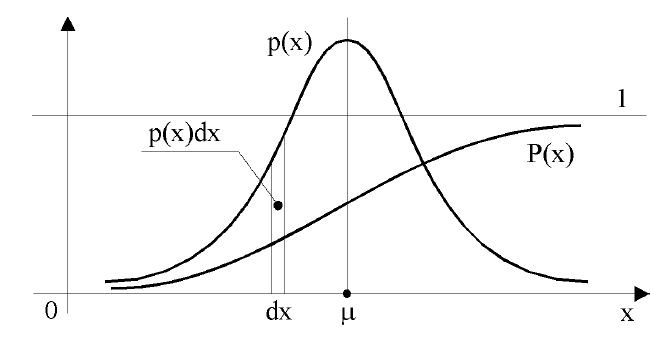
\includegraphics[scale = 0.8]{Curva di Gauss.png}
\end{figure}

\newpage 

\begin{tcolorbox}
    Argomento critico e importante nel corso. \newline

    La GUM, per quanto riguarda le misure, è la bibbia per chi fa misure, 
    quindi se non sai questo capitolo, meglio non svolgere l'esame in generale. \newline 
    
    La norma che andiamo a studiare è da 15 anni circa in vigore, 
    ma, adesso è in revisione. \newline 

    L'importante, anche durante l'esame scritto, sono i passaggi matematici che si svolgono. 
\end{tcolorbox}

\section{Regole di scrittura delle unità di misura}
\footnote{Slide della prof | SDME 2 Incertezza secondo GUM parte I | pag 2 - 4 \\  
Appunti | 2025-03-05 | pag 2 - 3}

Per questioni di praticità, sono stati introdotti i multipli ed i sottomultipli decimali delle unità di misura 
dell'SI, che si ottengono utilizzando i seguenti prefissi: 

\begin{figure}[h]
    \centering
    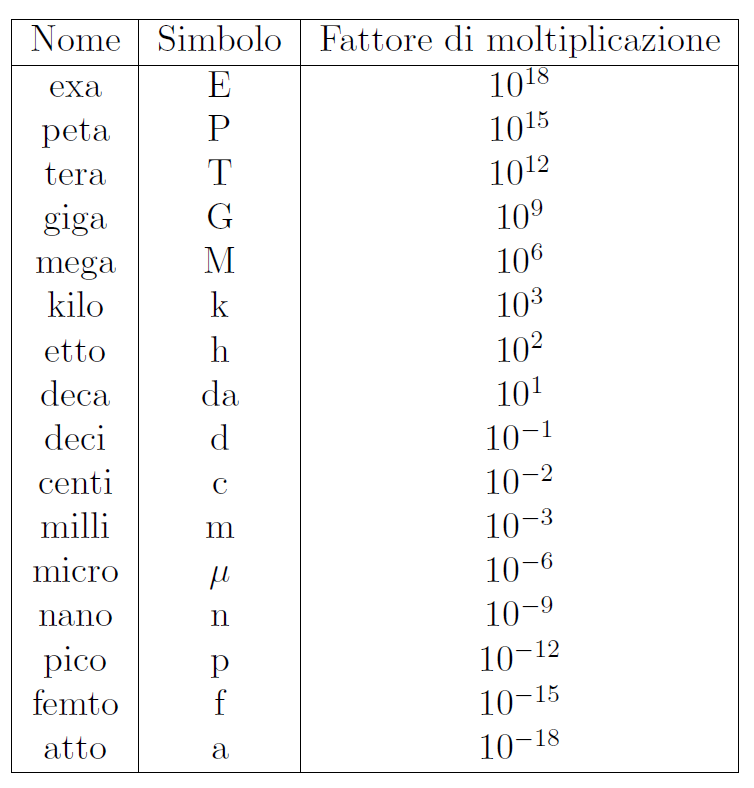
\includegraphics[scale = 0.5]{Tabella mutlipli e sottomultipli.png}
\end{figure}

Il simbolo di un multiplo o di un sottomultiplo di un'unità di misura 
si forma anteponendo il prefisso al simbolo dell'unità di misura. \newline 

Ad esempio: 

\begin{figure}[h]
    \centering
    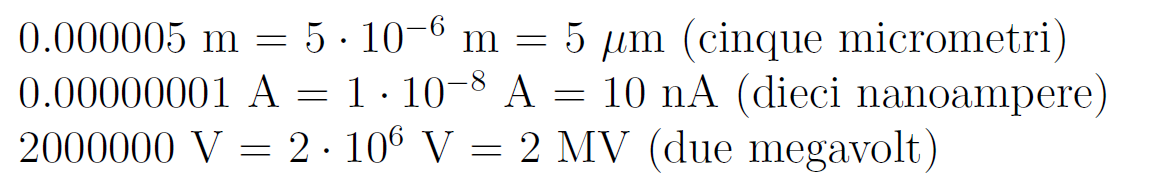
\includegraphics[scale = 0.3]{Esempi di conversione secondo GUM.png}
\end{figure}

Non è ammesso l'uso di prefissi composti, ad esempio: 

{
    \Large 
    \begin{equation}
        5 \text{ } pF \neq 5 \text{ } mnF
    \end{equation}
}

Prendendo come esempio l'u.d.m. del peso, cioè il grammo (g), 
i multipli ed i sottomultipli dell'unità fondamentale kilogrammo si formano a partire dal simbolo grammo. \newline 

Per esempio, si scrive: 

{
    \Large 
    \begin{equation}
        1 \text{ } mg \textbf{ NON } 1 \mu kg
    \end{equation}
}

Quando si fornisce il risultato di una misurazione, 
devono essere riportate soltanto le cifre significative, 
per cui è opportuno ricorrere ai multipli e sottomultipli delle unità SI per evitare ambiguità. \newline 

Nella seguente tabella, ci sono degli esempi: 

\begin{figure}[h]
    \centering
    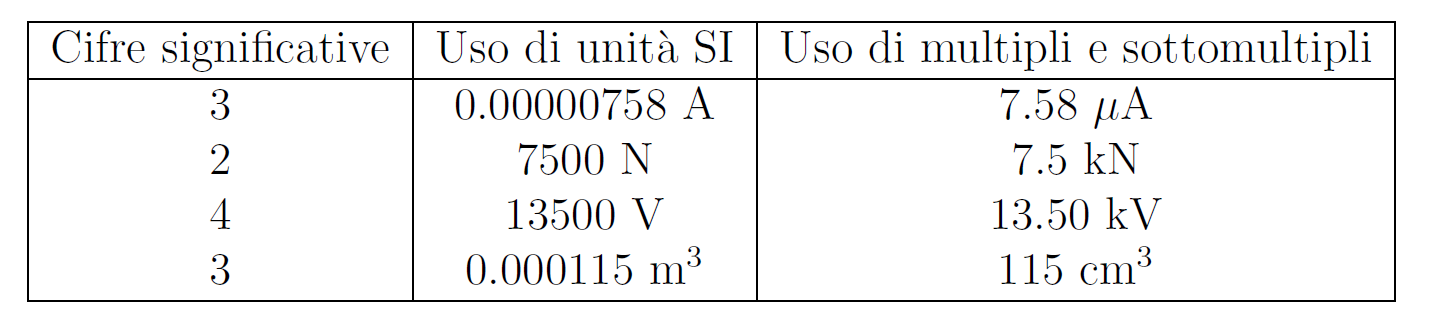
\includegraphics[scale = 0.3]{Esempio di cifre significative.png}
\end{figure}

I nomi delle unità SI, dei multipli e dei sottomultipli sono nomi comuni, 
per cui devono essere scritti con l'iniziale minuscola. \newline 

Si scriverà: 

\begin{itemize}
    \item ampere NON Ampere 
    \item kelvin NON Kelvin 
    \item gigahertz NON Gigahertz 
    \item gigahertz NON GigaHertz
\end{itemize}

Anche i simboli delle unità di misura sono scritti con l'iniziale minuscola, 
tranne quelli derivanti da nomi propri. \newline 

Quindi si scrivere: 

\begin{itemize}
    \item s per secondo 
    \item m per metro 
    \item C per coulomb 
    \item J per joule 
\end{itemize}

I nomi di tutte le unità SI e dei corrispondenti multipli e sottomultipli sono invariabili 
al plurale, eccetto per il metro, il kilogrammo, il secondo, la candela, la mola, il radiante e lo steradiante. \newline 

Il radiante e lo steradiante vengono utilizzati per esprimere i piani di una sfera. \newline 

Quindi è corretto scrivere: 

\begin{itemize}
    \item decine di metri 
    \item centinaia di volt, NON centinaia di volts 
    \item alcuni radianti 
    \item pochi kelvin, NON pochi kelvins
\end{itemize}

I simboli delle unità di misura devono essere scritti in carattere dritto normale, 
non devono essere seguiti da punti, tranne il caso in cui si trovano alla fine di un periodo, 
e devono seguire sulla stessa linea il valore numero che esprime la misura. \newline 

Quindi, è corretto $7.5$ V e NON V $7.5$. \newline 

Quando un'unità non accompagna la relativa misura, 
deve essere espressa con il suo nome e non con il suo simbolo. \newline 

Si scrive: 

\begin{itemize}
    \item il secondo è la durata NON il s è la durata 
    \item una lunghezza di alcuni metri e NON una lunghezza di alcuni m
\end{itemize}

I simboli di un'unità derivata ottenuta dal prodotto di due o più unità fondamentali
si indica interponendo il punto di moltiplicazione o uno spazio tra i simboli delle unità fondamentali. \newline 

Si scrive, ad esempio, 
N $\cdot$ m oppure N m .\newline 

Nel caso di unità derivate ottenute dal rapporto tra unità fondamentali, 
il simbolo dell'unità derivata si indica interponendo tra i simboli a numeratore e quelli a denominatore 
la barra obliqua o la riga di frazione. \newline 

In alternativa, possono essere usati gli esponenti negativi. \newline 

Si scrive, ad esempio J/s, m $\cdot$ $s^{-1}$. \newline 

\newpage 

\section{Unità non SI ammesse}
\footnote{Slide della prof | SDME 2 Incertezza secondo GUM parte I | pag 5 \\  
Appunti | 2025-03-05 | pag 3}

Alcune unità di misura non SI sono, per ragioni storiche, largamente utilizzate in campo scientifico, 
tecnico, commerciale e nella vita comune. \newline 

L'uso di queste unità è ammesso, MA non incoraggiato; 
inoltre, è sconsigliato associare unità SI e unità non SI. \newline 

La seguente tabella riporta alcune delle unità non SI ammesse: 

\begin{figure}[h]
    \centering
    \includegraphics[scale = 0.3]{Alcune unità non SI ammesse.png}
\end{figure}

\newpage 

\section{Il processo reale di misurazione e la definizione di "Misura"}
\footnote{Slide della prof | SDME 2 Incertezza secondo GUM parte I | pag 6 \\  
Appunti | 2025-03-05 | pag 3}

La definizione di misura data dalla norma UNI 4546 è una informazione costituita 
da un valore, una incertezza ed una unità di misura, segnata a rappresentare un parametro in un determinato stato del sistema. \newline 

Degli esempi di misure: 

\begin{figure}[h]
    \centering
    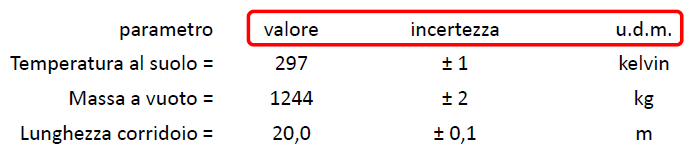
\includegraphics[scale = 0.5]{Esempi di misure.PNG}
\end{figure}

\newpage 

\section{La norma internazionale}
\footnote{Slide della prof | SDME 2 Incertezza secondo GUM parte I | pag 7 - 8 \\  
Appunti | 2025-03-05 | pag 4}

L'incertezza del risultato di una misurazione costituisce la mancanza di una conoscenza esatta del misurando. \newline 

Così, il risultato di una misurazione, quand'anche riuscissimo a correggere effetti sistematici identificati, 
costituisce sempre una stima del valore del misurando. \newline 

Il valore centrale è quello che noi scegliamo, indicando il suo intervallo perché 
il "valore vero" starà nell'intervallo. \newline 

L'incertezza sperimentale è dovuta a numerosi fattori, tra i quali: 

\begin{itemize}
    \item Definizione incompleta del misurando, imperfetta realizzazione del misurando 
    \item Distorsione personale dell'operatore nella lettura di strumenti analogici 
    \item Valori non esatti dei campioni e dei materiali di riferimento
\end{itemize}

Tutti questi fattori, inoltre, non sono sempre indipendenti, ma, 
in questo corso, li consideriamo indipendenti perché i calcoli sono molto più semplici. \newline 

Per questi fattori che possono "disturbare" la misura, anche se la GUM è breve, 
diventa molto più lunga a causa delle appendici con tutti i casi particolari. \newline 

\newpage 

\section{Approccio classico Vs GUM}
\footnote{Slide della prof | SDME 2 Incertezza secondo GUM parte I | pag 9 \\  
Appunti | 2025-03-05 | pag 5}

Analizzeremo la differenza tra errore, che è l'approccio classico, e l'incertezza, che è l'approccio della GUM. \newline 

Quando si parla di incertezza, ci si riferisce alla sola componente casuale. \newline 

Si dà per scontato che, se si mette in evidenza un effetto sistematico, 
questo vada corretto \textbf{PRIMA} di effettuare delle misure, e tale correzione sarà affetta anch'essa da una incertezza. \newline 

Nell'approccio classico, ci si riferisce all'origine dell'incertezza, 
mentre la divisione data nella GUM riguarda i metodi di valutazione dell'incertezza. \newline 

\newpage 

\section{Incertezza: altre considerazioni}
\footnote{Slide della prof | SDME 2 Incertezza secondo GUM parte I | pag 10 \\  
Appunti | 2025-03-05 | pag 5}

Alcune note riguardando l'incertezza. \newline 

Solo le definizioni hanno incertezza nulla. \newline 

C'è una incertezza intrinseca, la quale è la minima incertezza che può essere assegnata nella misura di un parametro, 
fissato un modello descrittivo della grandezza. \newline 

Spesso le prestazioni degli strumenti e dei campioni sono esuberanti rispetto ai requisiti necessari per la misura. \newline 

\newpage 

\subsection{Categorie di incertezza}
\footnote{Slide della prof | SDME 2 Incertezza secondo GUM parte I | pag 11 - 13 \\  
Appunti | 2025-03-05 | pag 5 - 6 | 2025-03-07 | pag 2}

La GUM classifica le componenti di incertezza in due categorie, 
in relazione al metodo di valutazione: 

\begin{itemize}
    \item Componenti valutate con metodi statistici (detti di tipo A), sono incertezze di misura che sono basati su metodi statistici, quindi oggettivi, perché la misura può essere ripetuta 
    \item Componenti valutate con altri metodi (detti di tipo B): si svolgerà una valutazione di tipo soggettivo perché la misura non può essere ripetuta
\end{itemize}

La regola di base è quella di fare, se possibile, almeno 3 misure. \newline 

La classificazione non indica alcuna differenza tra la natura delle componenti di incertezza. \newline 

I componenti di tipo B, generalmente, vengono basati sulla "bravura" dell'operatore. \newline 

È importante sottolineare che se il numero di ripetizioni della misura è relativamente ridotto, si fa più affidamento all'incertezza di tipo B. \newline 

Sia nelle categoria di tipo A e di tipo B, l'incertezza è valutata tramite una distribuzione di probabilità e la relativa deviazione standard. \newline 

Il principio base dell'approccio della GUM è che ogni componente di incertezza che contribuisce all'incertezza 
del risultato di misura è rappresentabile dalla stima del suo scarto tipo, 
chiamata incertezza tipo (che è indicata con la lettera u dall'inglese uncertainty) ed è uguale alla radice quadrata positiva della stima della varianza. 

\begin{tcolorbox}
    Tranquilli, nelle prossime sezioni sarà spiegato meglio con delle formule matematiche
\end{tcolorbox}

Se durante la misura tutte le grandezze d'influenza da cui essa dipende variano in modo casuale, 
si può utilizzare un approccio di tipo statistico, quindi di tipo A. \newline 

In diversi casi, ripetere le misure è una operazione lunga e costosa, non sempre fattibile. \newline 

Quindi, l'incertezza finale sulla misurazione è ottenuta sia dall'incertezza di tipo A e di tipo B. \newline 

\newpage 

\section{Alcuni richiami di statistica e probabilità}
\footnote{Slide della prof | SDME 2 Incertezza secondo GUM parte I | pag 14 - 16 \\  
Appunti | 2025-03-05 | pag 6 - 10 | 2025 -03-07 | pag 3}

\begin{tcolorbox}
    Sono gli stessi concetti di probabilità studiati a Teoria dei Segnali / Segnali Determinati Aleatori con il mitico Chiaraluce 
    ma applicati e adattati alla teoria delle misure
\end{tcolorbox}

Prendiamo in considerazione un indice quadratico, la varianza. \newline 

Definiamo varianza sperimentale dell'insieme di N misure il valore medio del quadrato delle deviazioni: 

{
    \Large 
    \begin{equation}
        \begin{split}
            s^{2} (x_k) 
            &= 
            \frac{1}{N - 1}
            \sum_{k = 1}^{N}
            \delta^{2}_k
            \\
            &= 
            \frac{1}{N - 1}
            \sum_{k = 1}^{N}
            (x_k - \overline{x})^{2}
        \end{split}
    \end{equation}
}

dove: 

\begin{itemize}
    \item $\overline{x}$ è la media dei valori 
    \item $x_k$ è il singolo valore della misura
\end{itemize}

Si pone $(x_k - \overline{x})^{2}$ elevato alla seconda perché $\delta_k$ può essere sia positivo che negativo. \newline

Da questa varianza, si deduce lo scarto tipico sperimentale come: 

{
    \Large 
    \begin{equation}
        \begin{split}
            s(x_k) 
            &=
            \sqrt
            { 
            \frac{1}{N - 1}
            \sum_{k = 1}^{N}
            \delta^{2}_k
            }
            \\
            &= 
            \sqrt
            {
            \frac{1}{N - 1}
            \sum_{k = 1}^{N}
            (x_k - \overline{x})^{2}
            }
        \end{split}
    \end{equation}
}

\newpage

\subsection{Scarto di tipo sperimentale}
\footnote{Slide della prof | SDME 2 Incertezza secondo GUM parte I | pag 17 \\  
Appunti | 2025-03-07 | pag 3 - 4}

Lo scarto tipo o deviazione standard rappresenta un indice appropriato della dispersione delle misure intorno al valore medio. \newline 

La sua definizione sarà, tuttavia, affinata, in seguito considerando che le N misure non rappresentano l'insieme (cioè la popolazione) di tutte 
le misure, 
ma solo un campione limitato dell'infinità di misure (teoricamente) eseguibili. \newline 

Utilizzando i diagrammi di Venn, possiamo rappresentare il caso della misura come:


%è la prima volta che provo a fare i disegni, sto seguendo questa guida: 
%https://latexdraw.com/how-to-draw-venn-diagrams-in-latex/

%E come al solito, Reddit salva la gente: 
%https://www.reddit.com/r/LaTeX/comments/o2367s/how_do_i_horizontally_centre_a_tikz_diagram/

% Circle with label
{
    \begin{center}
        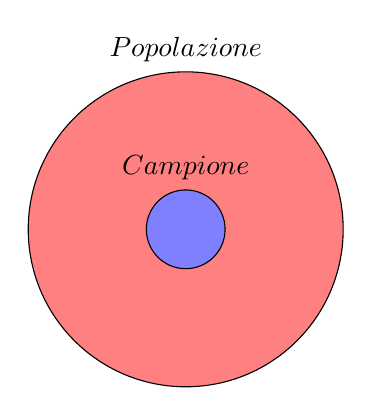
\begin{tikzpicture}
    
            \node[draw,
                circle,
                minimum size =4cm,
                fill=red!50,
                label=$Popolazione$] (circle1) at (0,0){};
            
            \node[draw, 
                circle, 
                minimum size = 1cm, 
                fill =blue!50, 
                label = $Campione$] (circle2) at (0,0) {};    
             
            \end{tikzpicture}    
    \end{center}
    
}

dove: 

\begin{itemize}
    \item nell'insieme della popolazione ci dovrebbero essere infiniti elementi 
    \item nell'insieme campione ci sono N elementi, quelli della misura
\end{itemize}

Quindi dagli elementi statistici utilizzati, e che hai imparato a conoscere al corso di teoria dei segnali con il mitico Chiaraluce, come: 

\begin{itemize}
    \item media $\mu$ 
    \item scarto (deviazione standard) $\sigma$
\end{itemize}

in una misura di N elementi utilizzeremo: 

\begin{itemize}
    \item media sperimentale $\overline{x}$ al posto di $\mu$ 
    \item deviazione scarto sperimentale $s(x_k)$ al posto di $\sigma$
\end{itemize}

\newpage 

\section{Istogrammi delle osservazioni}
\footnote{Slide della prof | SDME 2 Incertezza secondo GUM parte I | pag 18 - 21 \\  
Appunti | 2025-03-07 | pag 5}

Il risultato di numerose misure ripetute N sulla stessa grandezza 
possono essere graficamente rappresentati in opportuni diagrammi, 
detti istogrammi delle osservazioni come il seguente grafico: 

\begin{figure}[h]
    \centering
    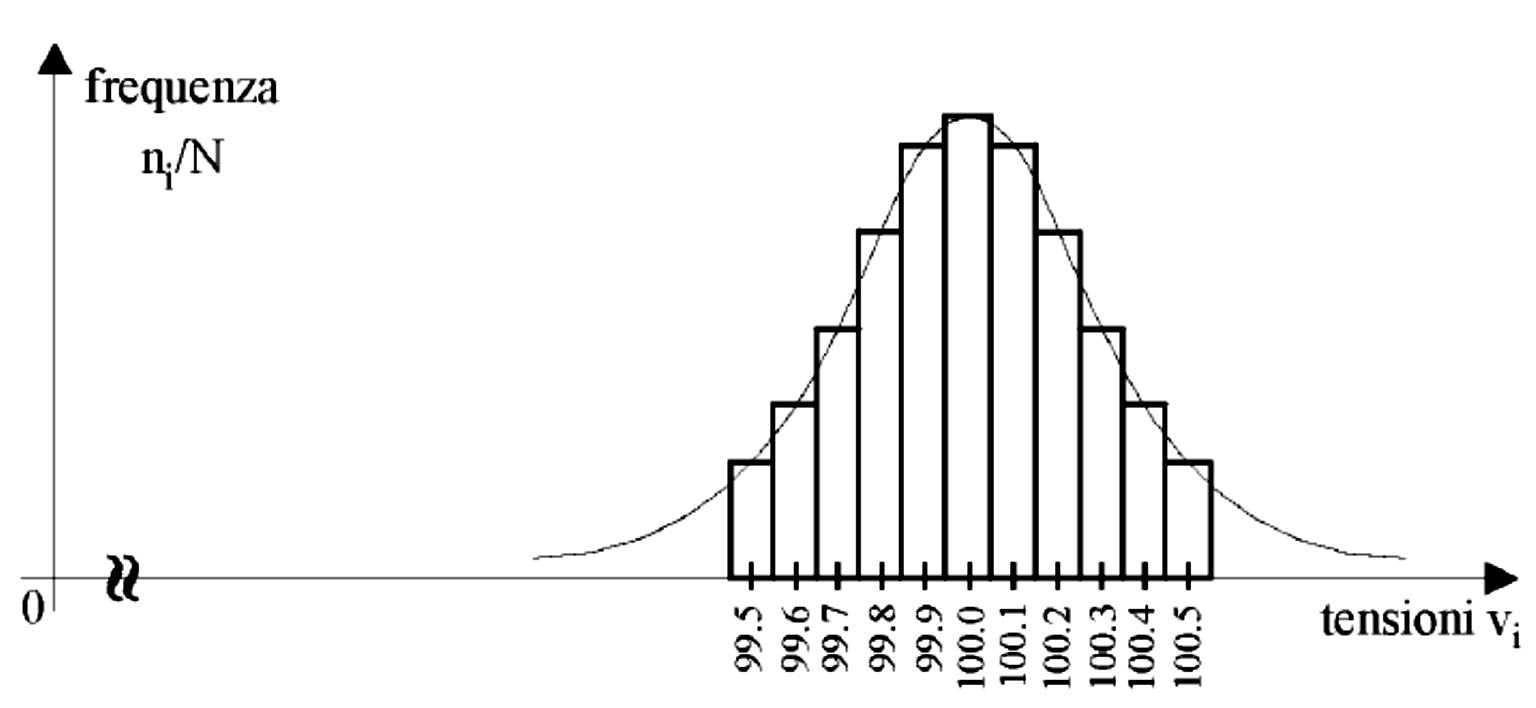
\includegraphics[scale = 0.2]{Esempio di istogramma delle osservazioni.png}
\end{figure}

Questi si costruiscono con alcune semplici operazioni: 

\begin{enumerate}
    \item Si individuano i valori massimo ($x_{max}$) e minimo ($x_{min}$) tra le N misure della grandezza X 
    \item Si divide l'intervallo ($x_{max} - x_{min}$) in un numero M di sotto-intervalli (chiamati in inglese bins) di uguale ampiezza, ciascuno dei quali può essere identificato col suo valore centrale \\ $x_i$ (i = 1, ..., M) 
    \item Si conta il numero $n_i$ delle misure che ricadono in ciascun sotto-intervallo 
    \item Si calcola la frequenza di osservazione dividendo questo numero per il numero totale delle osservazioni N: 
    {
        \Large 
        \begin{equation}
            f_i = \frac{n_i}{N} \text{ } (i = 1, 2, .., M)
        \end{equation}
    } 
    e, dalla teoria della probabilità: 

    {
        \Large 
        \begin{equation}
            \sum_{i=1}^{M}
            f_i 
            = 
            1
        \end{equation}
    }
\end{enumerate}

$f_i$ è la definizione frequentistica di probabilità. \newline 

Inoltre, la figura non è solo un istogramma, 
ma è un insieme tra istogramma, che è una funzione discreta, 
e una funzione normale continua, che è una astrazione matematica. \newline 
 
\newpage 

\section{Alcuni richiami di statistica e probabilità}
\footnote{Slide della prof | SDME 2 Incertezza secondo GUM parte I | pag 22 \\  
Appunti | 2025-03-07 | pag 6}

Con riferimento alle frequenze $f_i$, il valore medio è: 

{
    \Large 
    \begin{equation}
        \begin{split}
        \overline{x}
        &= 
        \frac{1}{N}
        \sum_{k = 1}^{N}
        x_k 
        \\
        &=
        \sum_{i = 1}^{M}
        x_i 
        \frac{n_i}{N} 
        \\ 
        &= 
        \sum_{i = 1}^{M}
        x_i f_i
        \end{split}
    \end{equation}
}

Invece la varianza si può scrivere come: 

{
    \Large 
    \begin{equation}
        \begin{split}
            s^{2} (x_i) 
            &= 
            \frac{1}{N - 1}
            \sum_{k = 1}^{N}
            \delta^{2}_k
            \\ 
            &= 
            \sum_{i = 1}^{M} 
            \delta^{2}_i 
            \frac{n_i}{N - 1}
            \\ 
            &= 
            \sum_{i = 1}^{M} 
            \delta^{2}_i 
            f^{\sim}_i
        \end{split}
    \end{equation}
}

in cui: 

{
    \Large 
    \begin{equation}
        \delta_i = x_i - \overline{x}
    \end{equation}
}

è lo scostamento della i-esima classe rispetto al valore medio. \newline 

M è il numero di valori distinti delle misure (cioè il numero di bins, dall'inglese "cestini"). \newline 

\newpage 

\section{Il concetto di probabilità ed i parametri statistici}
\footnote{Slide della prof | SDME 2 Incertezza secondo GUM parte I | pag 23 \\  
Appunti | 2025-03-07 | pag 6}

Se fosse possibile effettuare sulla stessa grandezza fisica X 
un numero N di misure infinitamente grande, 
le frequenze di occorrenza dei diversi valori rappresentano le probabilità dell'intera popolazione. \newline 

L'insieme delle misure può essere visto come una variabile aleatoria discreta X, 
dove ciascuno dei possibili valori $x_i$ è caratterizzato dalla sua probabilità di occorrenza: 

{
    \Large 
    \begin{equation}
        \begin{split}
            Prob(x_i)
            &= 
            P(x_i) 
            \\ 
            &=
            P_i 
            \\ 
            &= 
            \lim_{N \to \infty} 
            \frac{n_i}{N}
        \end{split}
    \end{equation}
}

Essendo un limite che tende ad infinito, nella realtà non si possono fare infinite misure: 
ecco perché viene utilizzata la statistica. \newline 

Molti fenomeni fisici, interessati solo da disturbi casuali, se osservati un numero di volte molto grande, 
obbediscono a una legge di occorrenza degli eventi detta Gaussiana o Normale. \newline 

\newpage 

\section{Curva normale o di Gauss}
\footnote{Slide della prof | SDME 2 Incertezza secondo GUM parte I | pag 24 \\  
Appunti | 2025-03-07 | pag 6}

Un esempio di curva normale o di Gauss: 

\begin{figure}[h]
    \centering
    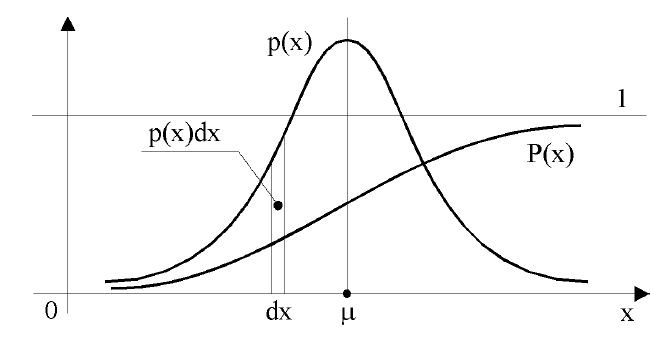
\includegraphics[scale = 0.4]{Curva di Gauss.png}
\end{figure}

Il diagramma della curva Normale o di Gauss per una variabile aleatoria continua X 
riporta in ascisse i possibili valori continui x della variabili aleatoria, 
mentre in ordinate si riporta la densità di probabilità p(x) con cui si osservano tali valori, 
e la probabilità cumulativa P(x). \newline 

\newpage

\section{Distribuzioni di probabilità}
\footnote{Slide della prof | SDME 2 Incertezza secondo GUM parte I | pag 25 - 27 \\  
Appunti | 2025-03-07 | pag 6 - 9}

La densità di probabilità p(x) è, in generale, quella funzione continua che, 
moltiplicata per una variazione infinitesima dx, fornisce la probabilità della variabile aleatoria X 
che cada dentro l'intervallo dx. \newline 

Quindi: 

{ 
    \Large 
    \begin{equation}
        Prob[x \leq X \leq (x + dx)]
        = 
        p(x) dx
    \end{equation}
}

La probabilità cumulativa P(x) è la probabilità che la variabile aleatoria X sia minore del valore corrente x: 

{
    \Large 
    \begin{equation}
        \begin{split}
            Prob [X < x]
            &= 
            P(x) 
            \\ 
            &= 
            \int_{- \infty}^{x}
            p(z) 
            dz 
        \end{split}
    \end{equation}
}

allora: 

{
    \Large 
    \begin{equation}
        \int_{- \infty}^{+ \infty} 
        p(x) dx 
        =
        1 
    \end{equation}
}

Invece si definisce valore medio come: 

{
    \Large 
    \begin{equation}
        \mu = \int_{- \infty}^{+ \infty} x \cdot p(x) dx
    \end{equation}
}

Si definisce varianza come: 

{
    \Large 
    \begin{equation}
        \sigma^{2}
        = 
        \int_{- \infty}^{+ \infty} 
        (x - \mu)^{2} \cdot p(x) dx
    \end{equation}
}

La radice quadrata della varianza è definita come scarto tipo o deviazione standard $\sigma$. \newline 

Talvolta, la densità di probabilità p(x) è riferita, anziché ai valori x delle misure, 
alle loro deviazioni $\delta = (x - \mu)$, tramite una semplice traslazione pari al valore medio. \newline 

Nella teoria della statistica, la gaussiana normale, quindi la gaussiana con area = 1, 
è molto utile per i calcoli, in particolare nelle misure può essere utilizzata per dimostrare la bontà della misura svolta. \newline 

Di seguito la densità di probabilità delle deviazioni standard normalizzata, la quale è diversa dalla densità di probabilità non normalizzata (perché l'area della funzione non è unitaria): 

\begin{figure}[h]
    \centering
    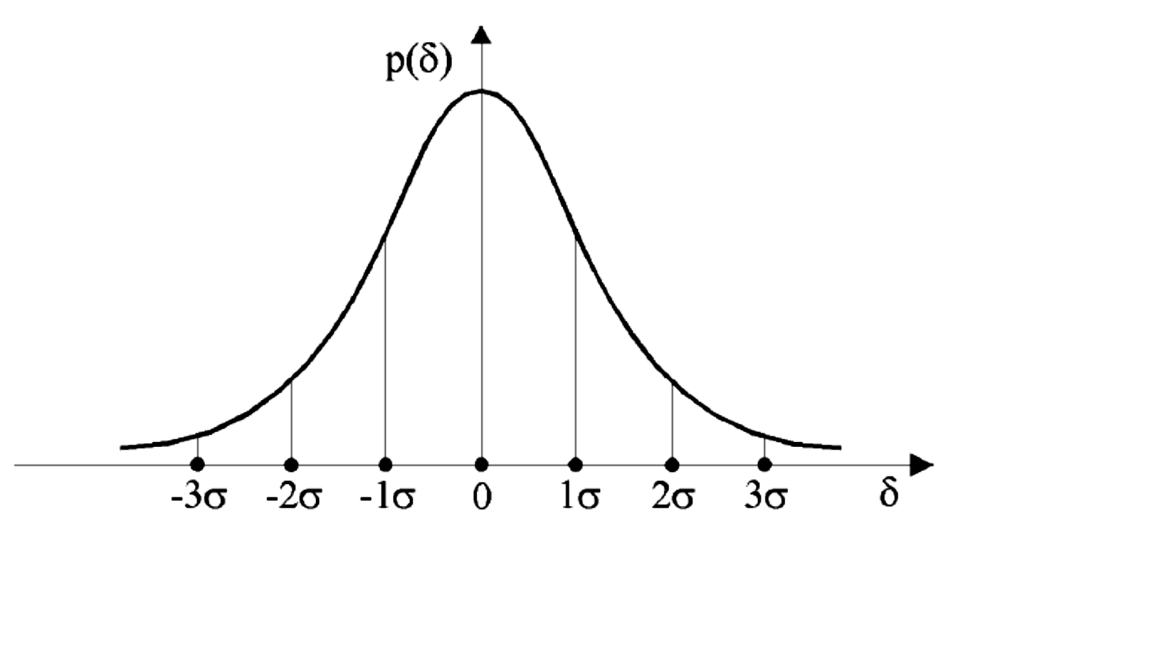
\includegraphics[scale = 0.4]{curva standard normalizzata di gaus.png}
\end{figure}

\newpage 

Si utilizza proprio una distribuzione di Gauss perché, da Segnali Determinati con Chiaraluce, 
il rumore ha questa distribuzione perché è un fenomeno stocastico. \newline 

Nella teoria delle misure e nella statistica, si divide la funzione gaussiana in $\sigma$ e suoi multipli. \newline 

Di seguito la relazione tra $\sigma$ e percentuale: 

{
    \Large 
    \begin{equation}
        Prob[- \sigma \leq \Delta \leq + \sigma] = 68.27 \%
    \end{equation}
}

{
    \Large 
    \begin{equation}
        Prob[- 2 \sigma \leq \Delta \leq + 2 \sigma] = 95.45 \%
    \end{equation}
}

{
    \Large 
    \begin{equation}
        Prob[- 3 \sigma \leq \Delta  \leq + 3 \sigma] = 99.73 \%
    \end{equation}
}


Assumendo l'intervallo $\pm 3 \sigma$ si avrà 99.73 \% che è circa 100 \% . \newline 

La bontà delle misure dipende dal suo scarto tipo: 
più è piccolo, meglio è perché la campana della gaussiana è più stretta. \newline 

Confrontando, ad esempio due misure di due laboratori: 

\begin{figure}[h]
    \centering
    \includegraphics[scale = 0.6]{Esempio bontà di misure.PNG}
\end{figure}

Le misure del laboratorio 1 sono di maggiori qualità rispetto al laboratorio 2 perché, 
riportando le densità di probabilità nelle distribuzioni normalizzate gaussiane, 
ci saranno più valori del laboratorio 1 rispetto alle misure del secondo laboratorio. \newline 

Per concludere, la densità di probabilità è un modello matematico, quindi non applicabile nella realtà perché N tende 
all'infinito, quindi useremo $s_k$ e i valori sperimentali. \newline 

\newpage 




